\section{MLOps: Despliegue y Puesta en Producción}
\label{sec:mlops}

El ciclo de vida del modelo culmina con su despliegue en un entorno de producción real, sustentado por una arquitectura de software robusta y procesos de gobernanza de código altamente automatizados.

\subsection{Arquitectura de Servicios e Idempotencia}
La pipeline de datos se ha diseñado siguiendo los principios \textbf{SOLID}, transformando scripts procedimentales en servicios especializados y desacoplados como \texttt{DatasetDownloader} y \texttt{DatasetProcessor}. Un pilar fundamental es la \textbf{idempotencia}: cada servicio verifica el estado del sistema antes de ejecutar operaciones costosas, optimizando el uso de recursos en la nube.

\subsection{Reproducibilidad y Gestión de Dependencias}
Para garantizar que el modelo se ejecute en entornos idénticos (local, AWS, Kubernetes), se utiliza el gestor \textbf{uv} y su archivo de bloqueo \textbf{\texttt{uv.lock}}. Esto asegura el determinismo absoluto del entorno, optimiza la caché de Docker y proporciona seguridad mediante la verificación de \textit{hashes} criptográficos.

\subsection{Optimización del Pipeline de CI: Eficiencia y Velocidad}
El flujo de integración continua en GitHub Actions se ha optimizado bajo dos vertientes: el tiempo de ejecución y el coste computacional.

\subsubsection{Estrategia de Caché Global con Fallback}
Dada la naturaleza pesada de las dependencias de Deep Learning, el sistema utiliza una caché compartida. GitHub Actions implementa una jerarquía donde el \textit{runner} busca primero en la rama actual y luego realiza un \textit{fallback} automático a \texttt{main}. Esto reduce el tiempo de build de 15 minutos a menos de 60 segundos.

\subsubsection{Validación Basada en Revisión (PR-driven CI)}
Se ha implementado una política de ejecución dirigida por \textbf{Pull Requests}. El pipeline de Docker solo se dispara cuando el código está listo para revisión, minimizando el consumo innecesario de recursos durante el desarrollo activo.

\subsection{Integridad del Código y Gobernanza mediante Rulesets}
Para asegurar la estabilidad de la rama principal (\texttt{main}), se ha configurado un \textbf{GitHub Repository Ruleset} que impone los siguientes controles de calidad:
\begin{itemize}
    \item \textbf{Fusión exclusiva vía PR:} Se prohíben los cambios directos en la rama principal, obligando a un proceso de revisión formal.
    \item \textbf{Status Checks Obligatorios:} El pipeline de construcción de Docker (\texttt{Docker Image CI}) debe finalizar con éxito antes de permitir cualquier integración.
    \item \textbf{Revisión Asistida por IA:} Se ha integrado \textbf{GitHub Copilot Code Review} de forma automática en el ruleset. Esto garantiza que cada cambio sea analizado por modelos de lenguaje avanzados para detectar vulnerabilidades, errores lógicos y asegurar el cumplimiento de las mejores prácticas antes de la intervención humana.
\end{itemize}

\subsection{Pruebas Automatizadas y Calidad de Código}
La fiabilidad se garantiza mediante una suite de pruebas con \texttt{pytest}, utilizando técnicas de \textit{mocking} para evitar dependencias externas. Estas pruebas se integran mediante \textit{hooks} de \textit{pre-commit}, manteniendo una cobertura superior al 95\%.

Para asegurar la correcta monitorización del despliegue en producción, se han establecido protocolos de depuración en tiempo real. Debido a que el proceso de descarga e inicialización del contenedor de Deep Learning puede demorar entre 3 y 6 minutos debido al volumen de las imágenes, se utiliza el sistema \texttt{cloud-init} para seguir el progreso del aprovisionamiento:

\begin{lstlisting}[language=bash, caption={Comando para monitorizar el aprovisionamiento inicial.}]
sudo tail -f /var/log/cloud-init-output.log
\end{lstlisting}

Una vez que el contenedor está activo, la trazabilidad del entrenamiento se mantiene mediante el acceso a los flujos de salida estándar de Docker, permitiendo una validación inmediata de la carga del modelo y la conexión con el sistema de persistencia en S3.

\subsection{Infraestructura como Código con Terraform}

La infraestructura de entrenamiento e inferencia se provisiona de forma reproducible mediante \textbf{Terraform} (versión del provider AWS \textasciitilde{}>5.0), con el estado remoto almacenado en un bucket S3 dedicado (\texttt{tfm-slm-terraform-state}, región \texttt{eu-south-2}) con cifrado en reposo y bloqueo de estado habilitados:

\begin{lstlisting}[language=hcl, caption={Configuración del backend remoto de Terraform.}]
backend "s3" {
  bucket       = "tfm-slm-terraform-state"
  key          = "terraform.tfstate"
  region       = "eu-south-2"
  encrypt      = true
  use_lockfile = true
}
\end{lstlisting}

El módulo de infraestructura provisiona cuatro recursos principales:

\begin{enumerate}
    \item \textbf{Instancia EC2 con GPU} (\texttt{g7e.2xlarge} por defecto): GPU NVIDIA RTX PRO Server 6000 (96 GB VRAM, arquitectura Ampere) con la AMI oficial de Amazon Deep Learning con drivers NVIDIA y PyTorch preinstalados. El \textit{UserData} de la instancia automatiza el bootstrap completo: actualización del sistema, descarga del código desde S3, compilación de la imagen Docker con soporte CUDA (incluyendo \texttt{flash-attn}) y lanzamiento del modo de operación seleccionado.

    \item \textbf{Buckets S3}: tres buckets con responsabilidades separadas --- \texttt{tfm-slm-code} para el ZIP del código fuente, \texttt{tfm-slm-checkpoints} para los pesos del modelo (con versionado habilitado), y \texttt{tfm-slm-benchmarks} para los resultados de evaluación en formato JSON.

    \item \textbf{Repositorio ECR} (\texttt{tfm-slm}): almacena la imagen Docker con \texttt{image\_tag\_mutability = MUTABLE} y política de ciclo de vida que retiene únicamente la última imagen, minimizando costes de almacenamiento.

    \item \textbf{Roles IAM}: el perfil de instancia \texttt{tfm-slm-ec2-profile} otorga a la EC2 permisos de \texttt{EC2ContainerRegistryPowerUser} y \texttt{S3FullAccess}, eliminando la necesidad de credenciales estáticas en el contenedor.
\end{enumerate}

\subsubsection{Pipeline de Despliegue}

El flujo de despliegue está orquestado por \texttt{deploy.py}, que actúa como punto de entrada único e interactivo. El operador selecciona el modo de operación (\texttt{train}, \texttt{inference} o \texttt{benchmark}), y el script ejecuta la siguiente secuencia de forma idempotente:

\begin{lstlisting}[language=bash, caption={Secuencia de despliegue desde la máquina local.}]
# 1. El operador lanza el script
python deploy.py          # selecciona modo (train/inference/benchmark)

# 2. deploy.py ejecuta automaticamente:
#    - archiva el codigo en tfm-slm-code.zip (sin __pycache__ ni ZIPs anteriores)
#    - sube el ZIP a s3://tfm-slm-code/
#    - verifica/crea el repositorio ECR
#    - verifica/crea el bucket de benchmarks

# 3. El operador aplica la infraestructura
cd app/terraform && terraform apply -auto-approve -lock=false

# 4. La EC2 arranca y ejecuta automaticamente build-and-train.sh
#    que construye la imagen Docker, la sube a ECR y lanza el modo elegido
\end{lstlisting}

El script \texttt{build-and-train.sh} ejecutado en la EC2 unifica los tres modos bajo la misma lógica: construcción de la imagen, push a ECR y lanzamiento del contenedor con la variable de entorno \texttt{MODE} correspondiente. El \texttt{entrypoint.sh} del contenedor enruta la ejecución al comando \texttt{uv} adecuado según el modo:

\begin{lstlisting}[language=bash, caption={Enrutamiento de modos en entrypoint.sh.}]
MODE=${MODE:-train}
if   [ "$MODE" = "inference"  ]; then tfm-slm-inference
elif [ "$MODE" = "benchmark"  ]; then tfm-slm-benchmark
else                                  tfm-slm
fi
\end{lstlisting}

Esta arquitectura permite cambiar entre entrenamiento, inferencia y benchmarking con un único parámetro, sin modificar la imagen Docker ni la infraestructura subyacente.

\subsubsection{Módulos Terraform: Configuración Detallada}

El código Terraform se organiza en seis módulos (archivos \texttt{.tf}), cada uno con responsabilidad específica. El directorio raíz (\texttt{app/terraform/}) contiene estos módulos, con una estructura modular que permite fácil extensión y auditoría.

\textbf{1. provider.tf: Configuración del Proveedor y Backend}

Define el proveedor AWS, la versión requerida, y el backend remoto para estado:

\begin{lstlisting}[language=hcl, caption={provider.tf: configuración de proveedor y backend remoto}]
terraform {
  required_providers {
    aws = {
      source  = "hashicorp/aws"
      version = "~> 5.0"
    }
  }
  backend "s3" {
    bucket       = "tfm-slm-terraform-state"
    key          = "terraform.tfstate"
    region       = "eu-south-2"
    encrypt      = true
    use_lockfile = true
  }
}

provider "aws" {
  region = var.aws_region
}
\end{lstlisting}

El backend S3 con \texttt{encrypt = true} proporciona protección en reposo. El \texttt{use\_lockfile = true} previene aplicaciones simultáneas que causarían corrupción de estado. La versión \texttt{\textasciitilde{}>5.0} asegura compatibilidad con APIs modernas de AWS sin versiones obsoletas.

\textbf{2. variables.tf: Parámetros Configurables}

Define variables de entrada que parametrizan la infraestructura, permitiendo diferentes configuraciones sin modificar código:

\begin{lstlisting}[language=hcl, caption={variables.tf: variables clave}]
variable "aws_region" {
  default = "eu-south-2"
}

variable "instance_type" {
  description = "EC2 instance type"
  default     = "g7e.2xlarge"
}

variable "deployment_mode" {
  description = "Deployment mode: train, inference, or benchmark"
  validation {
    condition = contains(["train", "inference", "benchmark"], var.deployment_mode)
    error_message = "deployment_mode must be 'train', 'inference', or benchmark'"
  }
}

variable "spot_price" {
  description = "Maximum price for Spot instance"
  default     = "1.50"
}
\end{lstlisting}

La variable \texttt{deployment\_mode} incluye validación (bloque \texttt{validation}) que rechaza valores inválidos en tiempo de plan, evitando errores de runtime.

\textbf{3. s3.tf: Buckets S3 y Versionado}

Provisiona buckets S3 para código, checkpoints, datasets y benchmarks. Ejemplo (checkpoints):

\begin{lstlisting}[language=hcl, caption={s3.tf: bucket con versionado para checkpoints}]
resource "aws_s3_bucket" "checkpoints" {
  bucket        = "tfm-slm-checkpoints"
  force_destroy = true
  tags = {
    Name        = "tfm-slm-checkpoints"
    Environment = "production"
  }
}

resource "aws_s3_bucket_versioning" "checkpoints" {
  bucket = aws_s3_bucket.checkpoints.id
  versioning_configuration {
    status = "Enabled"
  }
}
\end{lstlisting}

El versionado habilitado permite recuperar checkpoints anteriores si un entrenamiento diverge. El \texttt{force\_destroy = true} permite destruir el bucket (junto con contenido) via \texttt{terraform destroy}, útil para limpieza de desarrollo.

\textbf{4. ec2.tf: Instancia EC2, Security Groups, IAM Roles, AMI}

Es el módulo más complejo, provisioning la instancia GPU:

\begin{lstlisting}[language=hcl, caption={ec2.tf: seguridad y roles IAM (snippet)}]
# Security Group: permite SSH entrada
resource "aws_security_group" "ec2" {
  name        = "${var.project_name}-ec2-sg"
  vpc_id      = data.aws_vpc.default.id

  ingress {
    from_port   = 22
    to_port     = 22
    protocol    = "tcp"
    cidr_blocks = ["0.0.0.0/0"]
  }

  egress {
    from_port   = 0
    to_port     = 0
    protocol    = "-1"
    cidr_blocks = ["0.0.0.0/0"]
  }
}

# IAM Role: permisos ECR + S3
resource "aws_iam_role" "ec2_role" {
  name                = "${var.project_name}-ec2-role"
  assume_role_policy  = jsonencode({
    Version = "2012-10-17"
    Statement = [{
      Action = "sts:AssumeRole"
      Effect = "Allow"
      Principal = { Service = "ec2.amazonaws.com" }
    }]
  })
}

resource "aws_iam_role_policy_attachment" "ecr_power" {
  role       = aws_iam_role.ec2_role.name
  policy_arn = "arn:aws:iam::aws:policy/AmazonEC2ContainerRegistryPowerUser"
}

resource "aws_iam_role_policy_attachment" "s3_full" {
  role       = aws_iam_role.ec2_role.name
  policy_arn = "arn:aws:iam::aws:policy/AmazonS3FullAccess"
}
\end{lstlisting}

La instancia EC2 obtiene AMI Deep Learning via data source (busca la más reciente de Amazon):

\begin{lstlisting}[language=hcl, caption={ec2.tf: selección automática de AMI y lanzamiento}]
data "aws_ami" "dlami" {
  most_recent = true
  owners      = ["amazon"]
  filter {
    name   = "name"
    values = ["Deep Learning OSS Nvidia Driver AMI GPU PyTorch * (Amazon Linux 2023) *"]
  }
}

resource "aws_instance" "training" {
  ami                  = data.aws_ami.dlami.id
  instance_type        = var.instance_type
  iam_instance_profile = aws_iam_instance_profile.ec2_profile.name

  root_block_device {
    volume_size = 100
    volume_type = "gp3"
  }

  user_data = <<-EOF
    #!/bin/bash
    # Bootstrap: descarga codigo, construye Docker, inicia entrenamiento
    dnf update -y
    dnf install -y docker
    systemctl start docker
    aws s3 cp s3://tfm-slm-code/tfm-slm-code.zip .
    unzip tfm-slm-code.zip
    cd tfm-slm && docker build -t tfm-slm:latest .
    # ... mas comandos de inicializacion
  EOF
}
\end{lstlisting}

El \texttt{user\_data} es un script bash que se ejecuta automáticamente tras el boot de la instancia. Este script automatiza toda la secuencia: actualización del sistema, instalación de Docker, descarga de código desde S3, construcción de imagen, y lanzamiento del contenedor.

\textbf{5. ecr.tf: Repositorio ECR y Política de Ciclo de Vida}

Provisiona registro ECR con política de retención:

\begin{lstlisting}[language=hcl, caption={ecr.tf: repositorio ECR con garbage collection}]
resource "aws_ecr_repository" "main" {
  name                 = var.project_name
  image_tag_mutability = "MUTABLE"

  image_scanning_configuration {
    scan_on_push = true
  }

  force_delete = true
}

resource "aws_ecr_lifecycle_policy" "cleanup" {
  repository = aws_ecr_repository.main.name

  policy = jsonencode({
    rules = [{
      rulePriority = 1
      description  = "Keep only the last image to save space"
      selection = {
        tagStatus   = "any"
        countType   = "imageCountMoreThan"
        countNumber = 1
      }
      action = {
        type = "expire"
      }
    }]
  })
}
\end{lstlisting}

La política de ciclo de vida retiene únicamente la última imagen, evitando acumulación que incrementaría costos de almacenamiento ECR. El escaneo de imágenes (\texttt{scan\_on\_push = true}) detecta vulnerabilidades de seguridad automáticamente en cada push.

\textbf{6. outputs.tf: Valores de Salida}

Exporta información útil para usuarios/scripts posteriores:

\begin{lstlisting}[language=hcl, caption={outputs.tf: valores exportados tras provisioning}]
output "ec2_instance_id" {
  value = aws_instance.training.id
}

output "ecr_repository_url" {
  value = aws_ecr_repository.main.repository_url
}

output "s3_checkpoints_bucket" {
  value = aws_s3_bucket.checkpoints.bucket
}
\end{lstlisting}

Los outputs permiten que scripts externos (ej: \texttt{deploy.py}) obtengan IDs de recursos para operaciones post-provisioning sin re-descubrir via AWS CLI.

\textbf{Flujo de Ejecución Terraform}

El operador usa Terraform con esta secuencia:

\begin{lstlisting}[language=bash, caption={Operaciones Terraform típicas}]
# 1. Inicializar: descargar plugins, configurar backend
terraform init

# 2. Plan: visualizar que cambiara (sin aplicar)
terraform plan -var="deployment_mode=train"

# 3. Aplicar: provisionar recursos en AWS
terraform apply -auto-approve

# 4. Destruir: liberar recursos (limpieza)
terraform destroy -auto-approve
\end{lstlisting}

El \texttt{-auto-approve} acepta cambios sin confirmación interactiva, útil para CI/CD. Sin él, Terraform espera confirmación manual.

\subsubsection{Especificaciones de la Instancia EC2}

La instancia \texttt{g7e.2xlarge} provisiona los siguientes recursos de compute:

\begin{figure}[H]
    \centering
    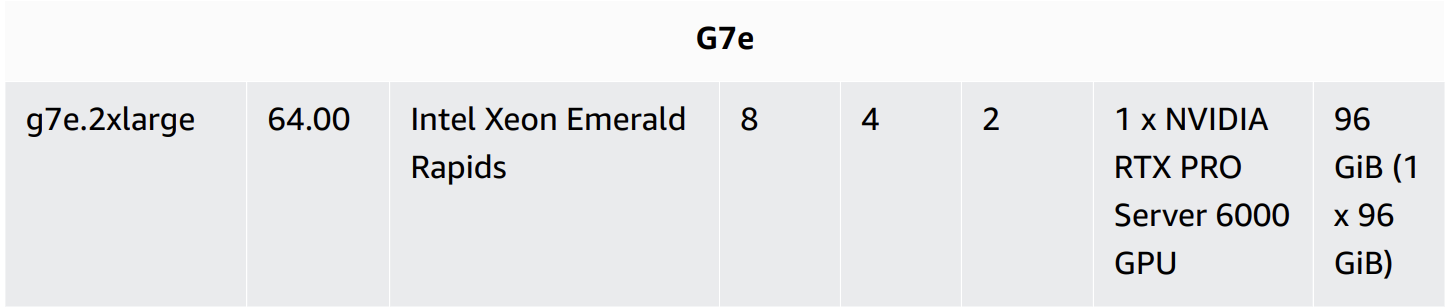
\includegraphics[width=0.95\textwidth]{images/aws_infrastructure/EC2_instance.png}
    \caption{Especificaciones de instancia EC2 g7e.2xlarge: 8 vCPUs (Intel Xeon Emerald Rapids), 64 GB RAM, NVIDIA RTX PRO Server 6000 con 96 GB VRAM. Esta configuración proporciona suficiente memoria para entrenar modelos de 124M parámetros con batch sizes de 64 tokens sin spilling a disco.}
    \label{fig:ec2_instance}
\end{figure}

\subsubsection{Visualización de Componentes AWS}

Los recursos de infraestructura se ilustran en las siguientes capturas, tomadas del panel de administración de AWS:

\begin{figure}[H]
    \centering
    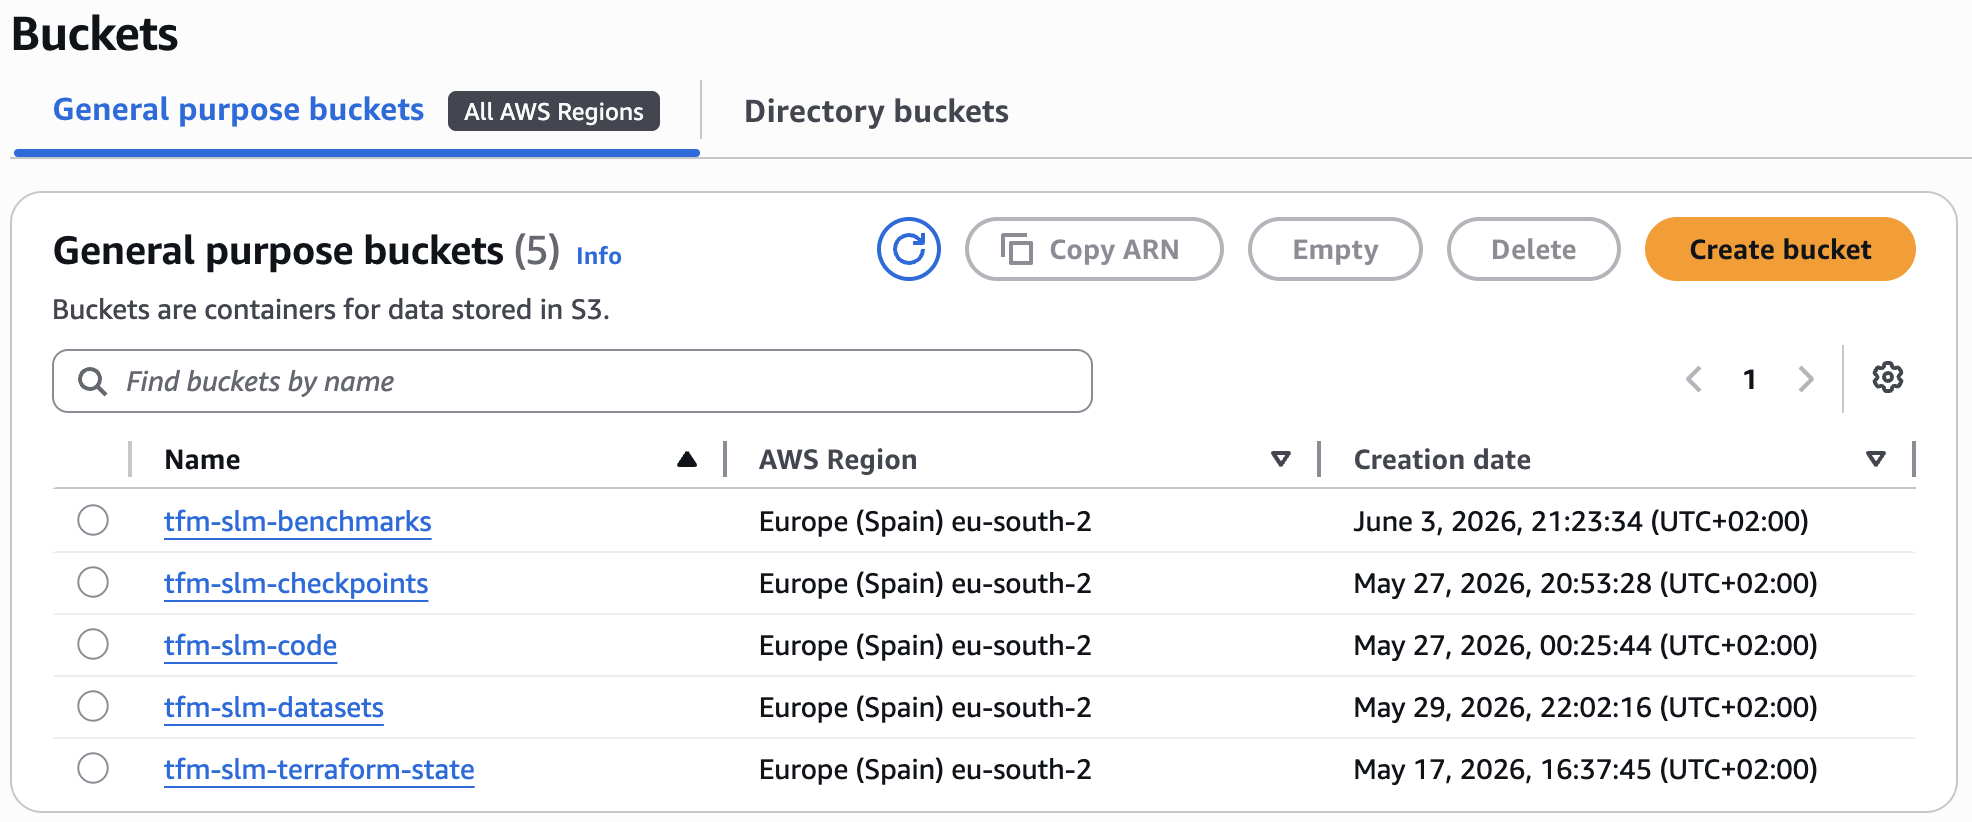
\includegraphics[width=0.9\textwidth]{images/aws_infrastructure/S3.png}
    \caption{Vista general de buckets S3 en AWS. El proyecto utiliza múltiples buckets con responsabilidades separadas: código fuente, checkpoints de modelo, datasets procesados, estado de Terraform, y resultados de benchmarking. Esta separación permite auditoría granular, políticas de ciclo de vida independientes y recuperación de desastres eficiente.}
    \label{fig:s3_general}
\end{figure}

\begin{figure}[H]
    \centering
    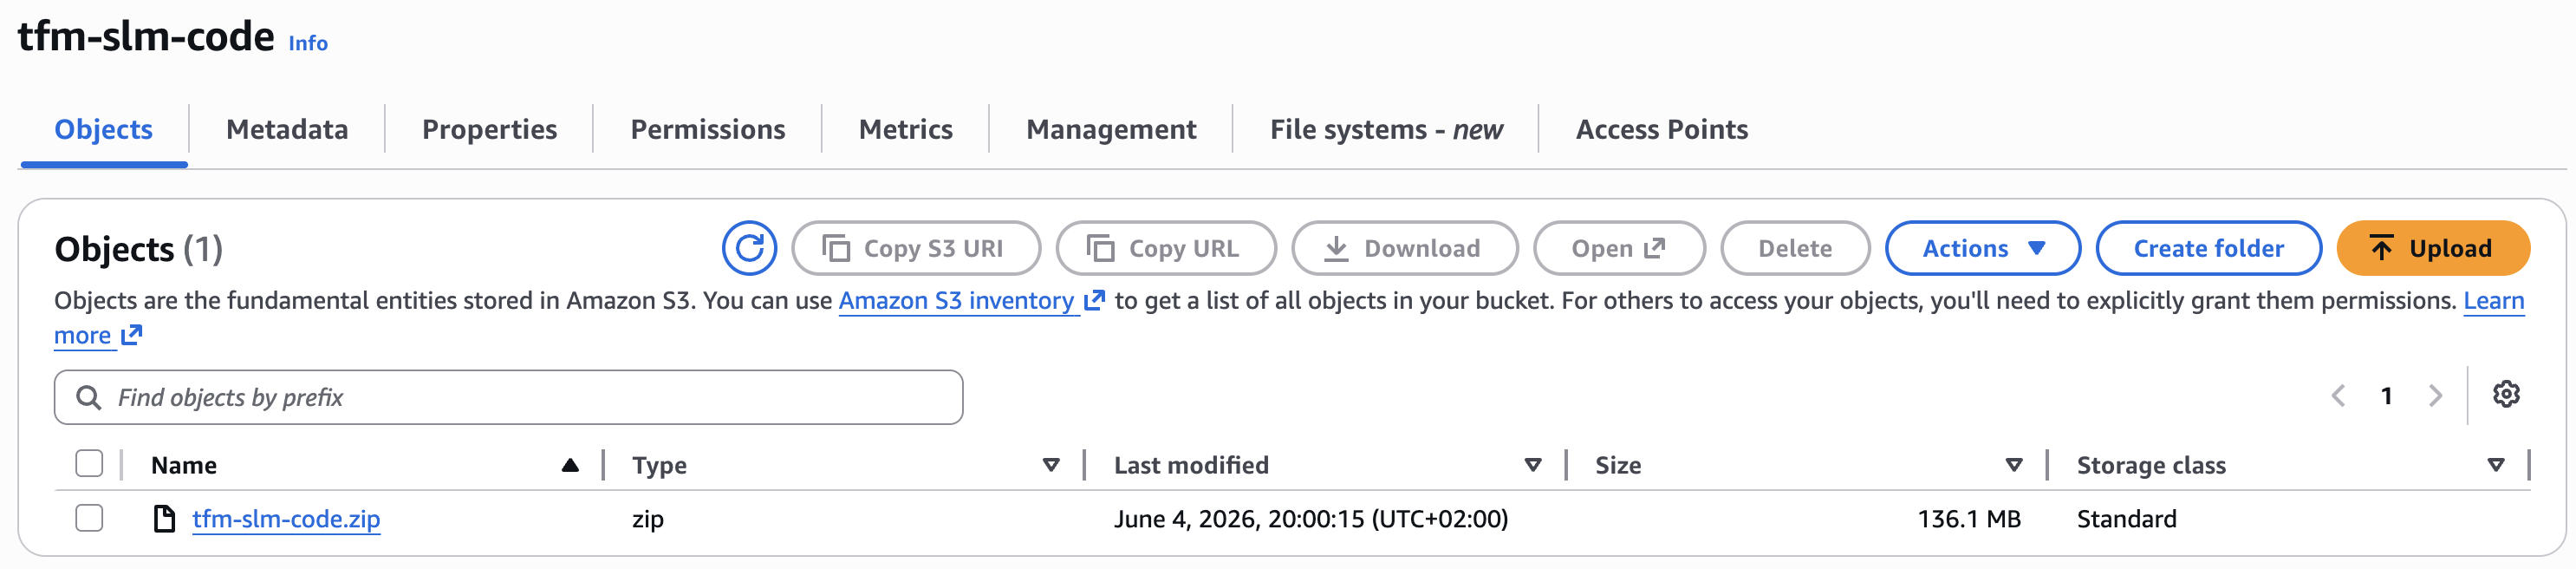
\includegraphics[width=0.9\textwidth]{images/aws_infrastructure/S3_code.png}
    \caption{Bucket S3 \texttt{tfm-slm-code}: almacena el ZIP del código fuente de la aplicación. El \textit{UserData} de la instancia EC2 descarga automáticamente esta fuente durante el bootstrap, permitiendo desacople entre gestión de infraestructura (Terraform) y gestión de código (Git/S3).}
    \label{fig:s3_code}
\end{figure}

\begin{figure}[H]
    \centering
    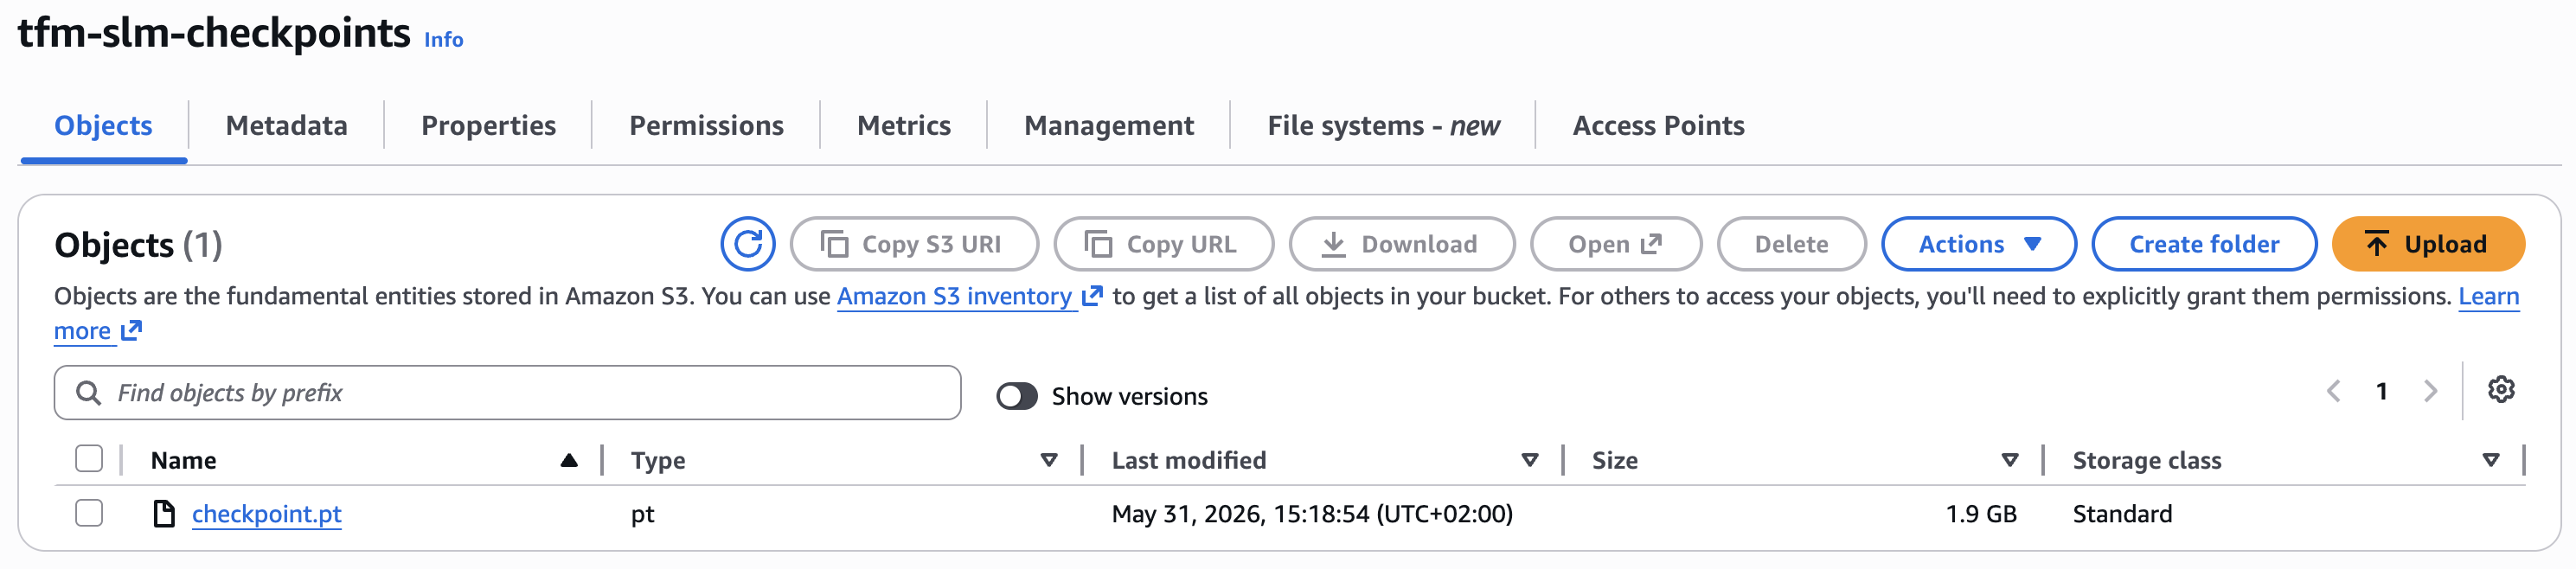
\includegraphics[width=0.9\textwidth]{images/aws_infrastructure/S3_chekpoints.png}
    \caption{Bucket S3 \texttt{tfm-slm-checkpoints}: almacena los pesos entrenados del modelo con versionado habilitado. Después de cada época, el entrenamiento guarda un checkpoint aquí, permitiendo reanudación si hay interrupciones. El versionado S3 proporciona auditoría completa de cambios y capacidad de rollback.}
    \label{fig:s3_checkpoints}
\end{figure}

\begin{figure}[H]
    \centering
    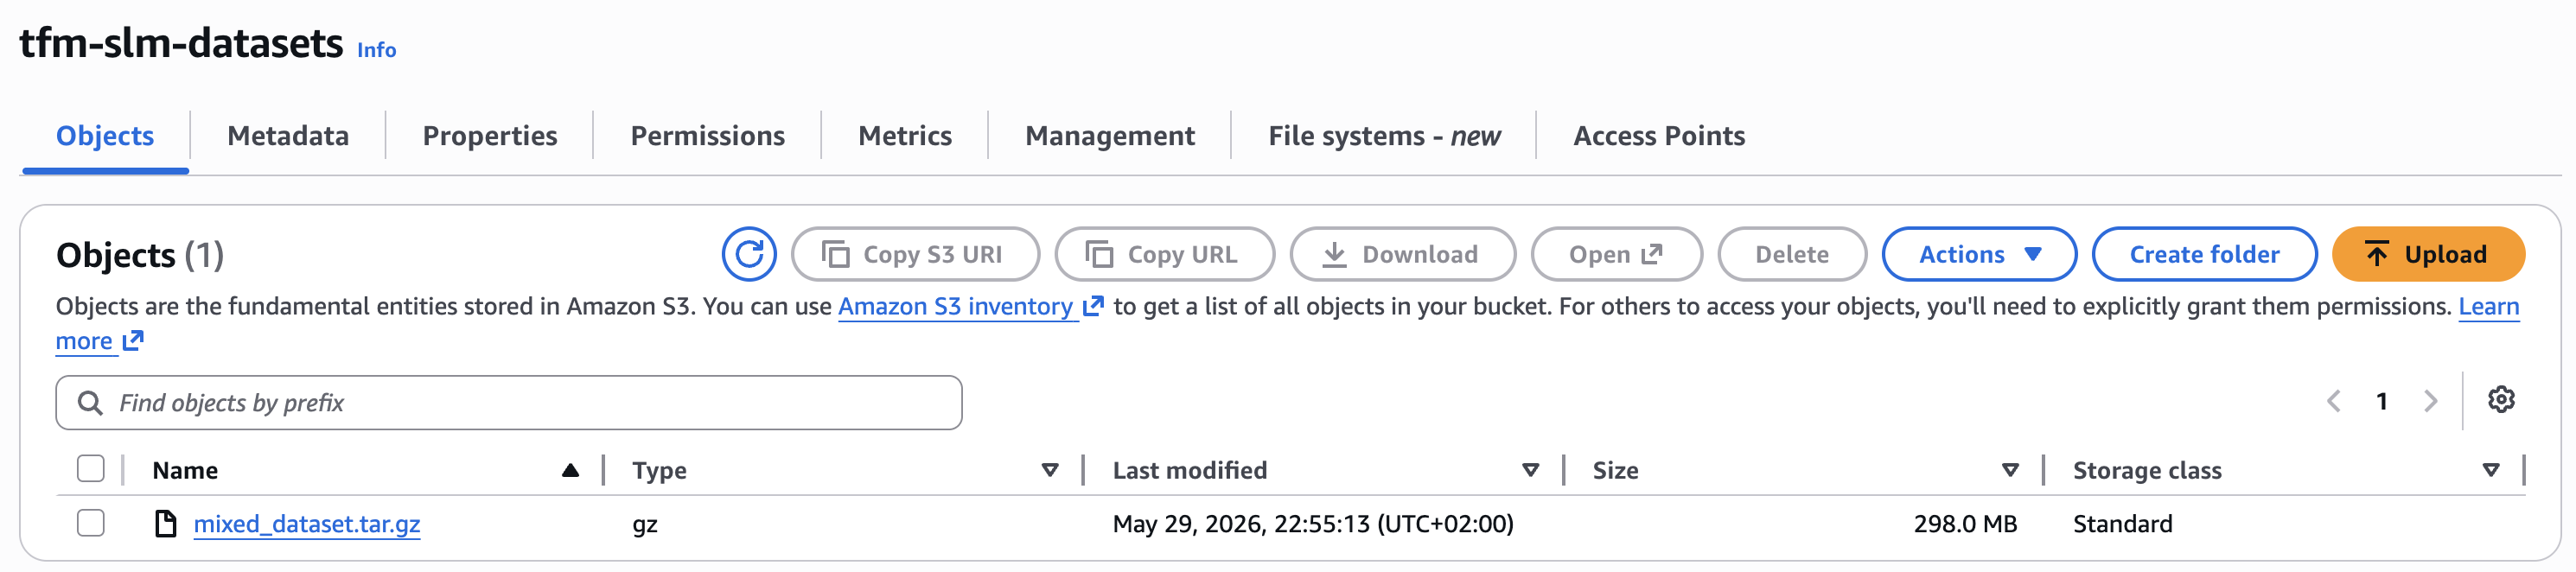
\includegraphics[width=0.9\textwidth]{images/aws_infrastructure/S3_datasets.png}
    \caption{Bucket S3 \texttt{tfm-slm-datasets}: almacena los datasets preprocessados en formato Apache Arrow. Durante la inicialización de la EC2, estos archivos se descargan y se cachean localmente en el almacenamiento de instancia, minimizando lectura repetida desde S3 durante entrenamientos de múltiples épocas.}
    \label{fig:s3_datasets}
\end{figure}

\begin{figure}[H]
    \centering
    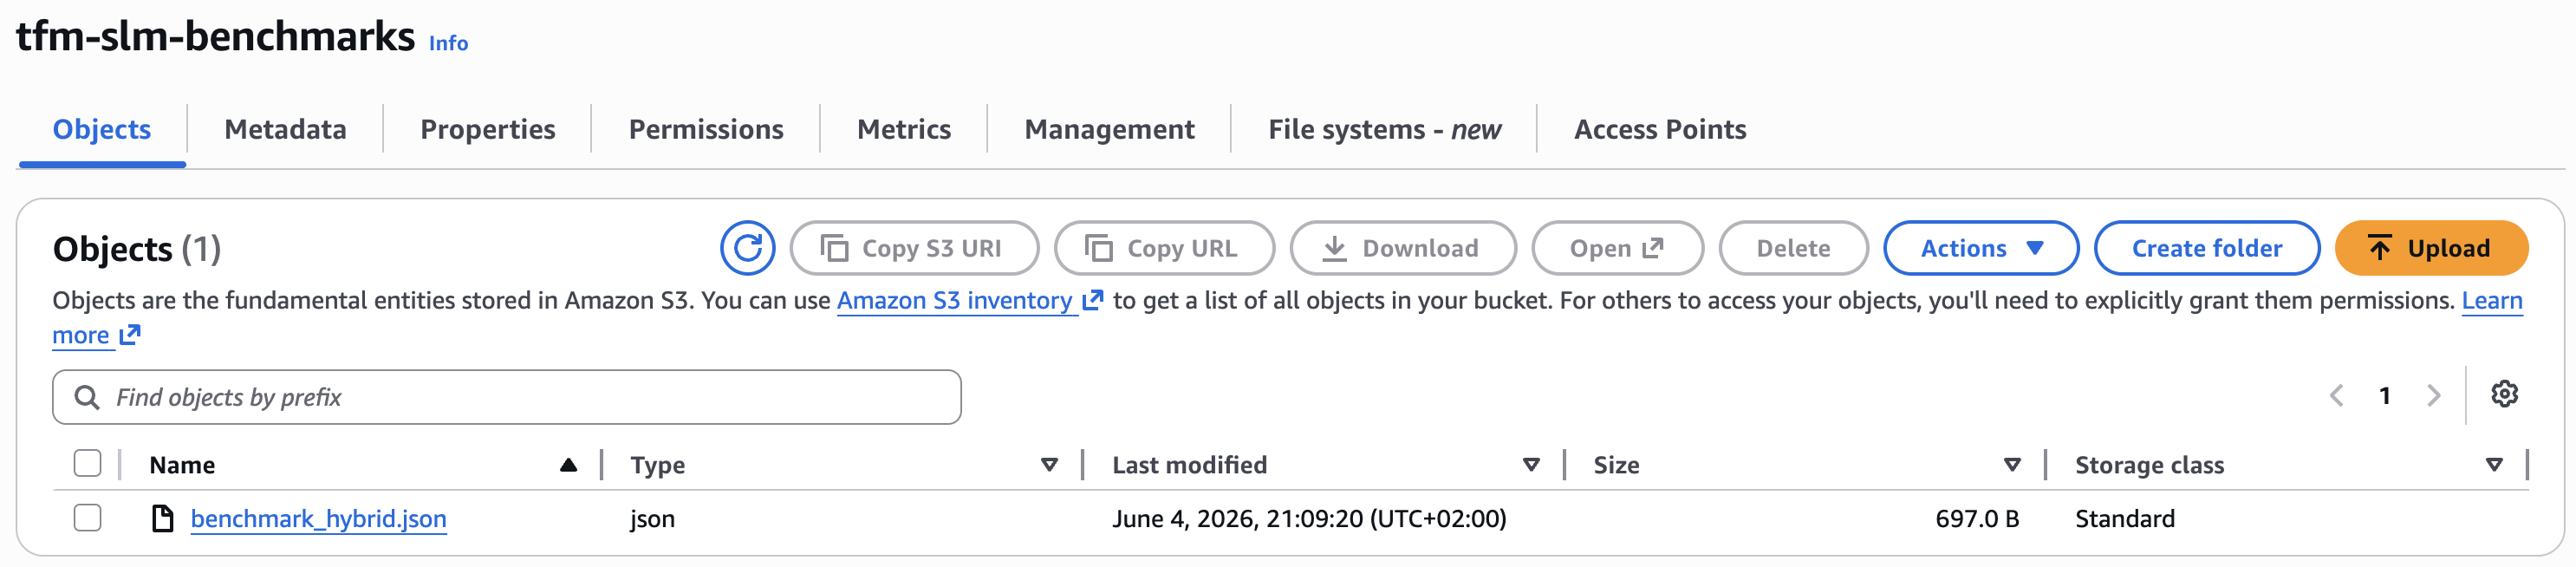
\includegraphics[width=0.9\textwidth]{images/aws_infrastructure/S3_benchmarks.png}
    \caption{Bucket S3 \texttt{tfm-slm-benchmarks}: contiene resultados de evaluación y benchmarking en formato JSON. Después de cada entrenamiento, métricas de perplexity, velocidad de inferencia y consumo de VRAM se exportan aquí, permitiendo análisis histórico y comparativas entre ejecuciones.}
    \label{fig:s3_benchmarks}
\end{figure}

\begin{figure}[H]
    \centering
    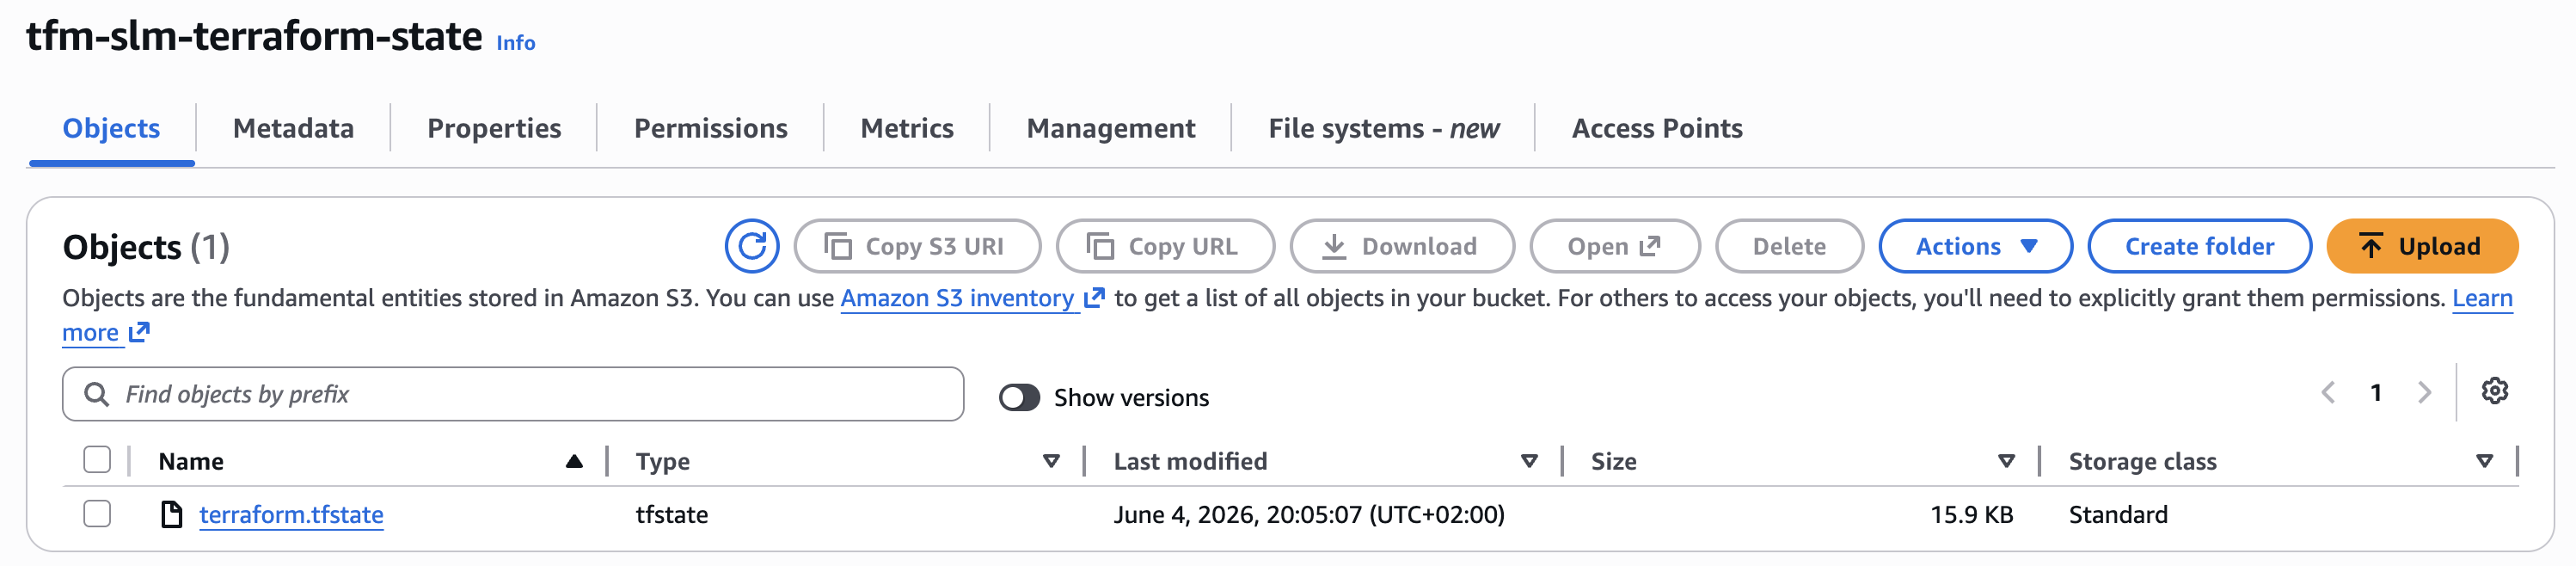
\includegraphics[width=0.9\textwidth]{images/aws_infrastructure/S3_terraform.png}
    \caption{Bucket S3 \texttt{tfm-slm-terraform-state}: almacena el archivo de estado de Terraform (\texttt{terraform.tfstate}) con cifrado en reposo y versionado. Este bucket se trata como crítico; su pérdida requeriría reconstrucción manual de toda la infraestructura. El bloqueo de estado (mutex) previene aplicaciones simultáneas que causarían corrupción de estado.}
    \label{fig:s3_terraform}
\end{figure}

\begin{figure}[H]
    \centering
    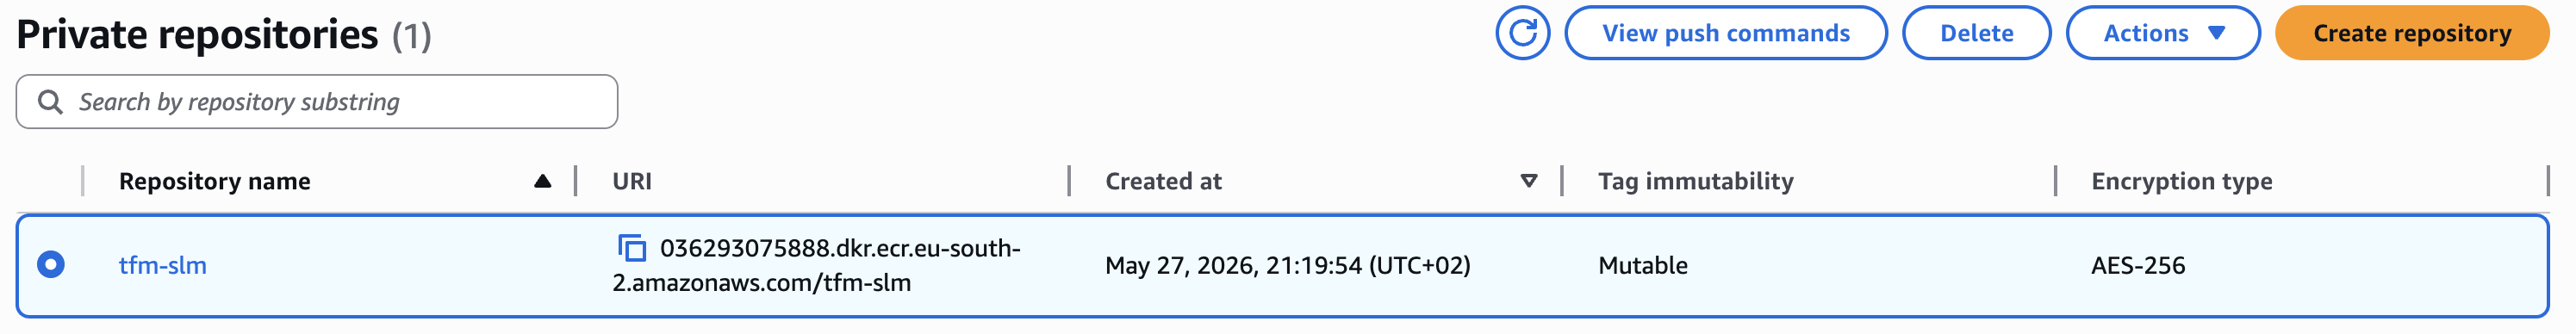
\includegraphics[width=0.9\textwidth]{images/aws_infrastructure/ECR.png}
    \caption{Elastic Container Registry (ECR) \texttt{tfm-slm}: repositorio privado de imágenes Docker. El pipeline de CI publica nuevas imágenes aquí después de cada build exitoso en GitHub Actions. La política de ciclo de vida retiene únicamente la última imagen, evitando acumulación de imágenes obsoletas y controlando costes de almacenamiento.}
    \label{fig:ecr}
\end{figure}

\begin{figure}[H]
    \centering
    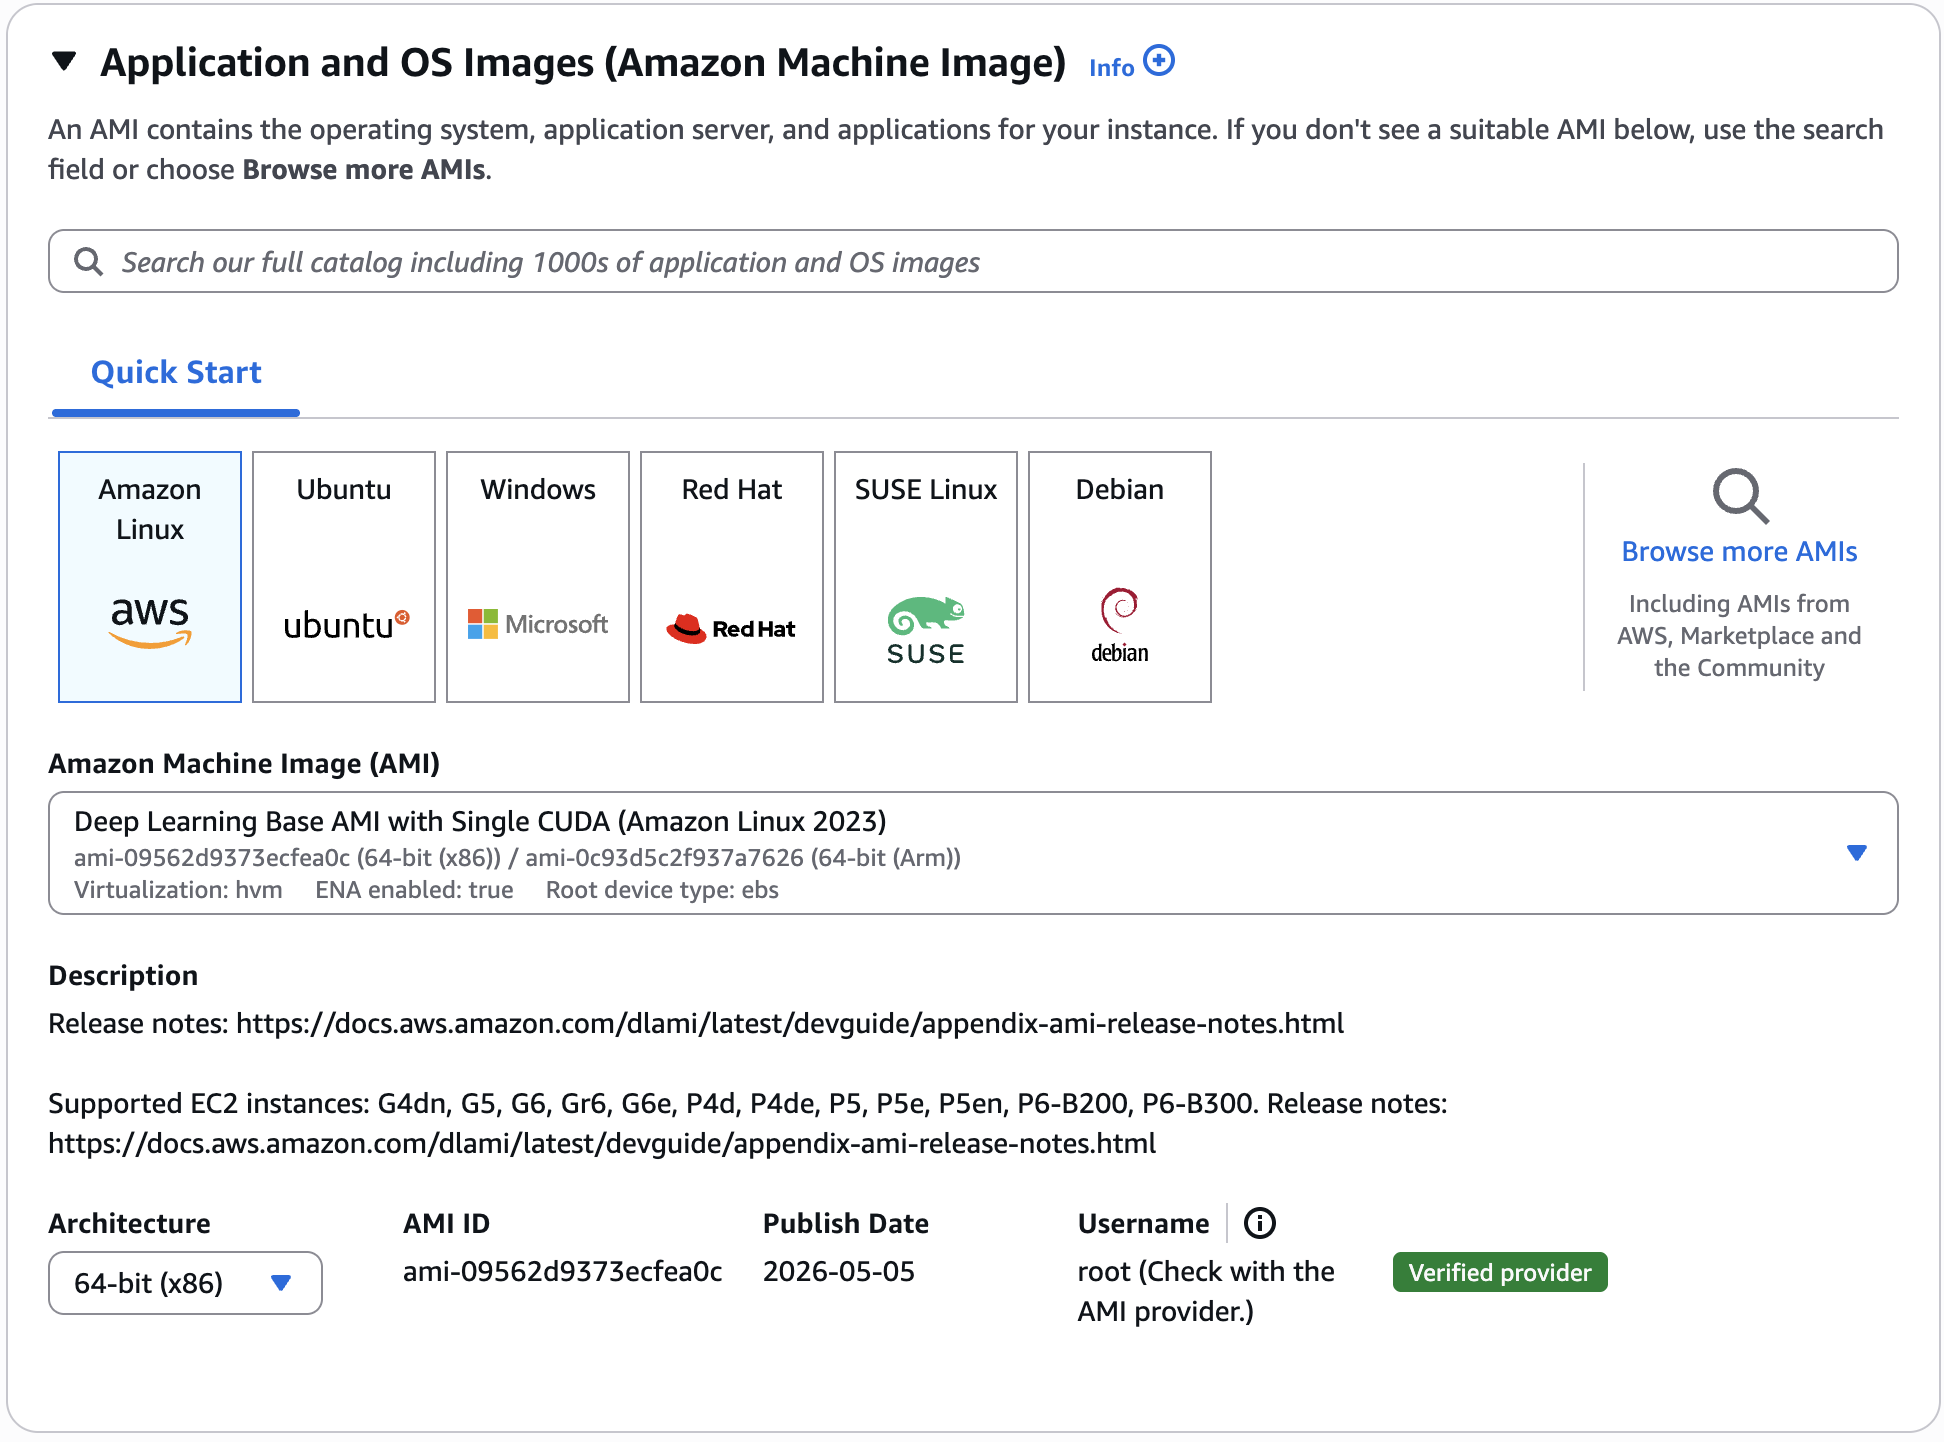
\includegraphics[width=0.9\textwidth]{images/aws_infrastructure/AMI.png}
    \caption{Amazon Machine Image (AMI) oficial de Deep Learning: preinstalada con drivers NVIDIA, CUDA, cuDNN y PyTorch. Usar esta AMI reduce el tiempo de bootstrap de la instancia EC2 de 20 minutos (compilación desde cero) a 3-6 minutos (solo descarga de contenedor y datasets). La AMI se especifica por ID en el módulo Terraform (\texttt{ami.tf}).}
    \label{fig:ami}
\end{figure}

\subsubsection{Topología y Flujo de Datos}

La arquitectura de AWS forma una topología donde S3 actúa como hub central:

\begin{enumerate}
    \item \textbf{Máquina Local} → \textbf{S3}: Desarrollador ejecuta \texttt{deploy.py}, que comprime código y lo sube a buckets S3 (\texttt{tfm-slm-code}, \texttt{tfm-slm-datasets}).

    \item \textbf{Terraform}: Lee estado desde \texttt{tfm-slm-terraform-state}, provisiona EC2 (con AMI Deep Learning), ECR, y roles IAM.

    \item \textbf{S3} → \textbf{EC2}: La instancia EC2 arranca y su script \textit{UserData} descarga código y datasets desde S3.

    \item \textbf{EC2} → \textbf{ECR}: En EC2, se construye imagen Docker (via \texttt{docker build}) y se sube a ECR como almacén central de imágenes.

    \item \textbf{EC2} (Contenedor): El contenedor (ejecutándose localmente en EC2, o descargado desde ECR) entrena el modelo. Periódicamente guarda checkpoints en S3 y exporta métricas a \texttt{tfm-slm-benchmarks}.

    \item \textbf{ECR}: Almacena imagen Docker construida como artifact reproducible para auditoría y futuros despliegues.
\end{enumerate}

Resumido: \textbf{S3 es el hub de entrada/salida}. Código y datasets fluyen desde S3 hacia EC2; checkpoints y métricas fluyen desde EC2 hacia S3. ECR es almacén de imagen Docker, no participa en flujo de datos de entrenamiento.

% ---------------------------------------------------------------
\subsection{Despliegue Local: Kubernetes con ArgoCD y Kustomize}

Mientras que el entrenamiento y benchmarking se ejecutan en infraestructura AWS bajo control de Terraform, la distribución del modelo entrenado para consumo por usuarios finales se realiza mediante un clúster Kubernetes local orquestado por ArgoCD. Este despliegue local proporciona un entorno aislado y reproducible donde desarrolladores e investigadores pueden interactuar con el modelo mediante una interfaz web integrada.

\subsubsection{Arquitectura del Clúster Local}

El clúster local se provisiona usando \textbf{Kind} (Kubernetes in Docker), ejecutando completamente dentro de contenedores sin dependencias de máquinas virtuales. La configuración se gestiona mediante \textbf{Kustomize}, que proporciona capacidades de parametrización declarativa sin necesidad de template engines como Helm.

Los componentes principales del despliegue son:

\begin{enumerate}
    \item \textbf{PersistentVolumeClaim} (\texttt{pvc.yaml}): Volumen local que almacena el checkpoint del modelo ($\sim$2 GB), permitiendo que los pods accedan al estado entrenado sin recargar desde red.

    \item \textbf{ConfigMap} (\texttt{configmap.yaml}): Variables de entorno de la aplicación, incluyendo la ruta del checkpoint (`/app/data/checkpoint.pt`) y configuración de memoria para CUDA.

    \item \textbf{Secrets} (\texttt{secrets.yaml}): Plantilla para credenciales de AWS (S3), permitiendo descargar modelos o logs desde la nube si es necesario.

    \item \textbf{Chat Deployment} (\texttt{chat-deployment.yaml}): Deployment de Kubernetes que ejecuta la aplicación de inferencia, exponiendo un servidor web en puerto 8000 con interfaz de chat y API REST.

    \item \textbf{Training Job} (\texttt{training-job.yaml}): Job de Kubernetes (opcional) que permite experimentar con entrenamiento en el clúster local utilizando GPU si está disponible.

    \item \textbf{Service} (\texttt{service.yaml}): Servicio de Kubernetes que expone el Deployment, permitiendo acceso interno dentro del clúster y port-forwarding hacia localhost.
\end{enumerate}

\subsubsection{Flujo GitOps con ArgoCD}

ArgoCD actúa como el \textbf{controlador de sincronización} entre el estado deseado (almacenado en Git bajo \texttt{argocd-cluster/manifests/}) y el estado actual del clúster. El manifiesto de aplicación ArgoCD (\texttt{application.yaml}) especifica:

\begin{lstlisting}[language=bash, caption={Configuración de sincronización GitOps en ArgoCD.}]
spec:
  source:
    repoURL: 'git://host.docker.internal/tfm_slm'
    path: argocd-cluster/manifests
  syncPolicy:
    automated:
      prune: true
      selfHeal: true
    syncOptions:
      - CreateNamespace=true
\end{lstlisting}

Las opciones de sincronización proporcionan:

\begin{itemize}
    \item \textbf{prune: true}: Si un recurso es eliminado de Git, ArgoCD lo elimina automáticamente del clúster.
    \item \textbf{selfHeal: true}: Si un pod muere o es modificado manualmente, ArgoCD lo restaura al estado deseado.
    \item \textbf{CreateNamespace: true}: Crea automáticamente el namespace \texttt{tfm-slm} si no existe.
\end{itemize}

\subsubsection{Ciclo de Despliegue Típico}

El flujo operacional para desplegar una nueva versión del modelo es:

\begin{enumerate}
    \item \textbf{Cambios en Git}: El usuario modifica los manifests en \texttt{argocd-cluster/manifests/} (ej: actualizar etiqueta de imagen, cambiar configuración de memoria).

    \item \textbf{Commit y Push}: Los cambios se commiterizean en el repositorio Git local (simulado con Git daemon en la máquina del desarrollador).

    \item \textbf{Detección de ArgoCD}: ArgoCD monitorea continuamente el repositorio y detecta divergencia entre Git y el clúster en menos de 3 segundos (configurable).

    \item \textbf{Sincronización Automática}: Sin intervención manual, ArgoCD aplica los cambios mediante \texttt{kubectl apply} automático, realizando \textit{rolling updates} de los pods sin downtime.

    \item \textbf{Rollback Inmediato}: Si hay problemas, la reversión se realiza simplemente haciendo revert del commit en Git; ArgoCD sincroniza nuevamente hacia el estado anterior.
\end{enumerate}

\subsubsection{Carga de Checkpoints y Uso Local}

Dado que el clúster Kind corre aislado dentro de Docker, el checkpoint debe transferirse explícitamente:

\begin{lstlisting}[language=bash, caption={Transferencia de checkpoint al clúster local.}]
# Obtener nombre del pod de chat
POD_NAME=$(kubectl get pods -n tfm-slm -l app=tfm-slm-chat \
           -o jsonpath='{.items[0].metadata.name}')

# Copiar checkpoint desde el Mac hacia el volumen persistente del pod
kubectl cp .output/checkpoint.pt tfm-slm/$POD_NAME:/app/data/checkpoint.pt

# Reiniciar el pod para que cargue el checkpoint
kubectl rollout restart deployment/tfm-slm-chat -n tfm-slm
\end{lstlisting}

Una vez reiniciado, el modelo está disponible para inferencia. Los usuarios pueden acceder mediante:

\begin{enumerate}
    \item \textbf{Interfaz Web}: Navegador en \texttt{http://localhost:8000}, proporcionando chat visual en tiempo real.
    \item \textbf{API REST}: Consultas directas con \texttt{curl} o clientes HTTP, permitiendo integración en aplicaciones externas.
\end{enumerate}

\subsubsection{Ventajas del Despliegue Local}

Este enfoque ofrece varias ventajas sobre un despliegue directo en la máquina local:

\begin{itemize}
    \item \textbf{Aislamiento}: El modelo corre en su propio namespace, sin contaminar dependencias del sistema operativo.
    \item \textbf{Escalabilidad}: Pasar de 1 a múltiples réplicas es trivial: cambiar \texttt{spec.replicas} en el manifest.
    \item \textbf{Reproducibilidad}: Cualquier desarrollador puede clonar el repositorio y desplegar la misma configuración.
    \item \textbf{Auditoría}: Toda decisión de despliegue queda registrada en el historial de Git.
    \item \textbf{Zero Downtime}: Las actualizaciones de imagen ocurren sin interrumpir el servicio gracias a rolling updates.
\end{itemize}